\section{Related Work}

Clustering tools often fall into two specific categories: \emph{hierarchical} or \emph{greedy}.
In this section, we will discuss each clustering paradigm and their popular implementations (Table \ref{table:clustering_tools}).

\subsection{Hierarchical clustering}
The traditional approach for clustering sequences was to use a hierarchical clustering method.
These methods start with a pair-wise distance matrix and then iteratively merge similar points into clusters.
Distance between two sequence can be the minimum number of edits (insertions, deletions, substitutions) to transform one sequence into the other (called \emph{edit distance}), the \emph{similarity} (defined as the $1 - \frac{\text{edit distance}}{|\text{sequence}|}$), and \emph{identity} (fraction of bases that are identical between the two sequences).
In addition to the above distances, we can create a vector of counts for all k-length substrings of the sequences (called \emph{k}-mers) and calculate some distance measure (such as euclidean) between the resulting vectors.

It is important to note that not all distance measures are created equally, though.
A distance metric must obey the triangle inequality, i.e., for every sequences \emph{A}, \emph{B}, and \emph{C}, $dist(A,B) + dist(B,C) \leq dist(A,C)$.
The identity measure does not follow the triangle inequality.

Once we have selected a distance measure, we need to calculate the pair-wise distances for all sequences to create our distance matrix.
Lets assume we have selected edit distance for our distance measure.
Edit distance between two sequences of length $n$ can be calculated via dynamic programming, a strategy for solving problems by breaking them down into ``simpler'' subproblems, in $O(n^2)$ time and work.
We will discuss the algorithms used in more detail in the next section.

Once the distance  is built, clustering is typically done via hierarchical methods.
Agglomerative methods involve a bottom-up approach, where each sequence starts as its own cluster then iteratively merged with other clusters.
Divisive methods, on the other hand, work from a top-down approach, where all sequences belong to a single cluster then are iteratively split into smaller clusters.

\subsection{Greedy clustering}

Calculating the pair-wise edit distance between $N$ sequences will take $O(N^2n^2)$ work.
This amount of time is impractical for the large number of sequences produced by sequencing technologies today.
454 sequencing by the 454 Life Sciences company can produce tens of millions of sequences.
An alternative approach to hierarchical clustering sequences involves iteratively selecting a sequence to serve as a cluster center and then recruiting all remaining sequences that fall within some given distance of the cluster center.
This process is repeated until no more sequences remain or the predetermined list of centers is exhausted.
In this section, we will discuss the different strategies for selecting centers and the heuristics used to speed up the alignment of sequences to centers.


%selecting a sequence from our database to serve as the cluster center.
%The center is then used to recruit the remaining sequences that fall within some given \emph{distance} threshold to the center using fast heuristics.

%A commonly-used clustering paradigm for sequence clustering is to iteratively select a sequence to serve as a cluster center and then recruit all remaining sequences that fall within some given distance of the cluster center.
%This process is repeated until no more sequences remain or the predetermined list of centers is exhausted.


%The time complexity of hierarchical clustering algorithms is 

%The traditional approach for clustering 16S rRNA sequences has involved the use of a multiple sequence alignment (MSA) for all sequences.

%Optimal multiple sequence alignment between a collection of sequences can be done with a dynamic programming algorithm.


%Greedy methods can be used to iteratively build a rooted tree.
%Then a specific cutoff can be given to split the tree into clusters.

%Alternatives include building a distance matrix between each pair of sequences.  

%While hierarchical methods requires less work than the multiple sequence alignment, calculating the pairwise distances generally requires cubic work, making it impracticable for a large number of sequences.


% Booktabs require to add \usepackage{booktabs} to your document preamble



%\subsection{Greedy clustering paradigm}

\begin{table}[t!]
\centering\scriptsize
\hspace*{-1.5cm}
\begin{tabular}{@{}llcccccccc@{}}
\toprule
Tool        & Description                                                                                                                                       & DNA & Protein & \emph{De novo} & Ref & Exact & Multi-core & Distance measure         & Strategy     \\ \midrule
BLAST\cite{altschul_gapped_1997}       & \multirow{4}[3]{4.5cm}{Alignment tool using neighborhood keywords to speed up alignment A script can be used to align to a reference database and filter results.}       & Y   & Y       & N       & Y             & N     & Y                & N/A                      & N/A          \\
\\
\\
\\
\\
\\
AbundantOTU\cite{ye_identification_2010} &  \multirow{2}[3]{4.5cm}{Fast method to build cluster centers from abundant k-mers}                                                                                         & Y   & N       & Y       & N             & Y     & N                & Sim               & Greedy       \\
\\
\\
\\
CD-HIT\cite{li_clustering_2001,fu_cd-hit:_2012}      &  \multirow{2}[3]{4.5cm}{Family of clustering tools. Speed comes from using a short word filter to prune potential alignments.}                                             & Y   & Y       & Y       & N             & N\tablefootnote{Only exact for a preset number of similarities.}    & Y                & Sim               & Greedy       \\
\\
\\
\\
DNACLUST\cite{ghodsi_dnaclust:_2011}    &  \multirow{2}[3]{4.5cm}{Fast, exact clustering tool that exploits database sequence similarity to reduce work.}                                                            & Y   & N       & Y       & Y             & Y     & Y                & Sim / Mis & Greedy       \\
\\
\\
\\
DySC\cite{zheng_dysc:_2012}        &  \multirow{2}[3]{4.5cm}{Uses a two-step clustering heuristic to build larger clusters.}                                                                                    & Y   & N       & Y       & N             & N     & N                & Sim               & Greedy       \\
\\
\\
ESPRIT-Tree\cite{cai_esprit-tree:_2011} &  \multirow{2}[3]{4.5cm}{Hierarchical method that represents a cluster of sequences as a single probabilistic sequence and uses that for pair-wise alignments of clusters.} & Y   & N       & Y       & N             & N\tablefootnote{Default k-mer length filter does not guarantee correctness.}     & N                & Sim               & Hierarchical \\
\\
\\
\\
\\
HPC-CLUST\cite{rodrigues_hpc-clust:_2014}   &  \multirow{2}[3]{4.5cm}{Scalable, and flexible hierarchical method for clustering pre-aligned reads.}                                                                      & Y   & N       & Y       & N             & N/A\tablefootnote{Takes as input pair-wise sequence distances.}    & Y                & Sim               & Hierarchical \\
\\
\\
\\
SEED\cite{bao_seed:_2011}        &  \multirow{2}[3]{4.5cm}{Very fast clustering of highly similar reads within 3 mismatches.}                                                                                 & Y   & N       & Y       & N             & Y     & N                & Mis               & Greedy       \\
\\
\\
UCLUST\cite{edgar_search_2010}      &  \multirow{2}[3]{4.5cm}{Fast clustering method that only compares a sequence to a predetermined number of potential centers.}                                              & Y   & Y       & Y       & Y             & N\tablefootnote{Default is inexact, but also offers an exact alignment mode.}    & Y                & Sim               & Greedy       \\ 
\\
\\
\\
\bottomrule
\end{tabular}
\caption{Clustering tools used in metagenomic studies. DNA and Protein refers to whether the clustering tool can work with DNA and protein sequences, respectively.  \emph{De novo} and Ref refers to whether the clustering tool can cluster sequences without and with a reference database, respectively. Exact clustering tools are those that compare a sequence to every cluster center. Multi-core clustering tools are those that support multiple threads.  Distance measure refers to tools that define distance between two sequences as percent similarity or mismatch number.  Strategy defines how the centers are created with greedy methods having some fixed procedure of selecting the center from the dataset, while hierarchical refers to those that are constructed using a guide tree.}
\label{table:clustering_tools}
\hspace*{-1.5cm}
\end{table}



\subsubsection{Cluster center selection}
%This is the method used by CD-HIT\cite{li_clustering_2001,fu_cd-hit:_2012}, DNACLUST\cite{ghodsi_dnaclust:_2011}, UCLUST\cite{edgar_search_2010}, and SEED\cite{bao_seed:_2011}.

%CD-HIT\cite{li_clustering_2001,fu_cd-hit:_2012}, DNACLUST\cite{ghodsi_dnaclust:_2011}, and UCLUST\cite{edgar_search_2010}


There are three strategies used for selecting potential cluster centers: {\bf \emph{de novo}}, {\bf closed-reference}, and {\bf open-reference}.

In {\bf \emph{de novo}} clustering, centers are selected \emph{only} from the set of input sequences.
Selecting which sequence to use as the cluster center is a difficult problem.
One strategy is to select the remaining sequence with the longest length, as is done by CD-HIT\cite{li_clustering_2001}, DNACLUST\cite{ghodsi_dnaclust:_2011}, and UCLUST\cite{edgar_search_2010}.
An intuitive argument is that a longer sequence would more likely recruit shorter sequences.
However, the more rigorous argument is that selecting the longest remaining sequence allows you certain guarantees when aligning and recruiting shorter sequences.
For example, given 3 sequences: \emph{A}, \emph{B}, and \emph{C} (Figure \ref{fig:overlap}).  If the length of \emph{B} (our center) is less than \emph{A} and \emph{C} and we know \emph{dist(\emph{A},\emph{B})} and \emph{dist}(\emph{B}, \emph{C}), we can not say anything for certain about the \emph{dist}(\emph{A}, \emph{C}).
We do not have any data about the overlapping regions between \emph{A} and \emph{C} that extend past the end of \emph{B}.
As we will explain in the next section, this problem exists only for semi-global alignment where gaps at the start and end of the sequences are not penalized.  If we used global alignments then overhanging regions of \emph{A} and \emph{C} would be penalized.

In addition to sorting by length, UCLUST providers users with alternative methods for selecting the centers.
UCLUST assumes that the sequences are sorted in an order such that a \emph{good} centroid is found before other sequences in its cluster.
When sequences have a large variation in length, the recommended strategy is to sort the sequences by length first as with CD-HIT and DNACLUST.
However, it is possible to assign an abundance to each sequence prior to clustering.
The user can run a fast deduplication program prior to clustering to get a pseudo-cluster count prior to running UCLUST.

AbundantOTU\cite{ye_identification_2010} uses a different strategy to construct its cluster centers.
It starts by finding the most abundant \emph{k}-mer (called the seed).
Then the seed is greedily extended one nucleotide at a time, selecting the nucleotide that has the highest similarity with the input sequences that share the same seed.
AbundantOTU works well at assembling highly abundant OTUs because it is robust to sequencing errors.
Errors within OTUs should occur less frequently than their correct bases in abundant clusters.
The authors of AbundantOTU recommend using the tool to cluster the abundant OTUs than using another clustering strategy for the remaining sequences.

%UCLUST also allows users to select potential centers based on abundances.


\begin{figure}[tb!]
  \centering
    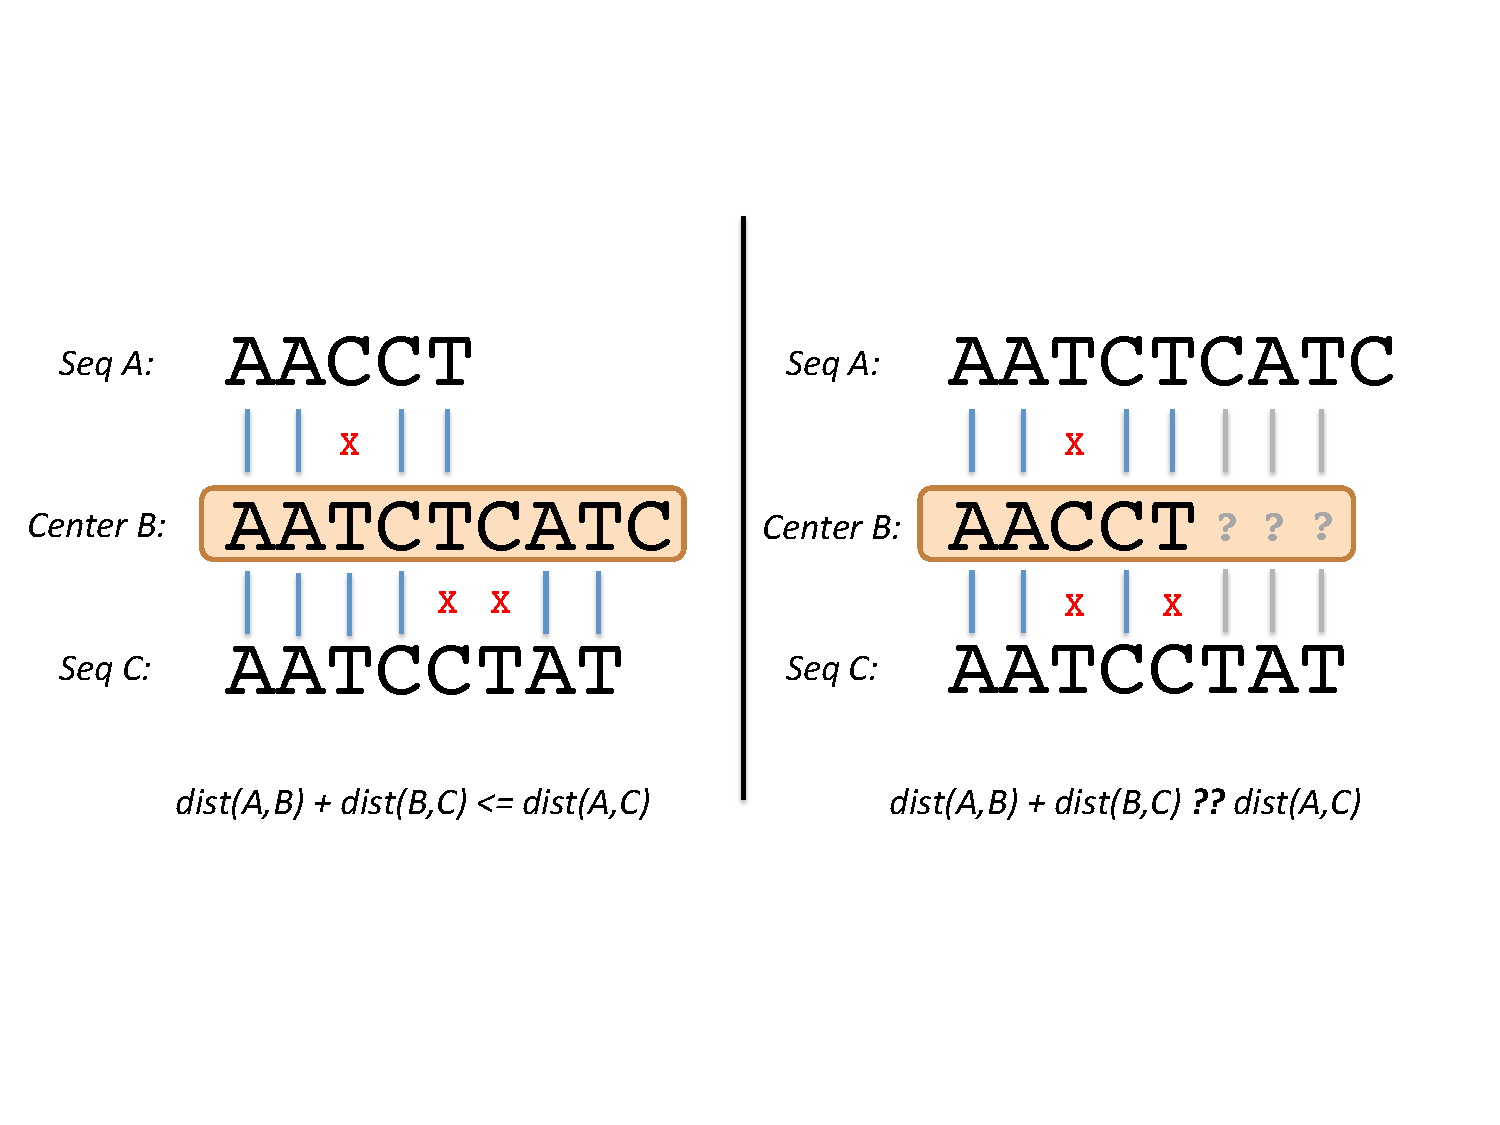
\includegraphics[width=0.7\textwidth]{overlap}
  \caption{The longest sequence is chosen as the center (left side) so that we can make transitive application of the distances of sequences within the cluster.  If the longest sequence is not chosen as the center (right side), then we can not make any claims about distance of the overhanging regions of other sequences in the cluster.}
  \label{fig:overlap}
\end{figure}



In {\bf closed-reference} clustering, a list of predetermined centers is given, such as a collection of previously discovered or manually-curated OTUs\cite{desantis_greengenes_2006,quast_silva_2013}.
16S rRNA pipelines such as QIIME\cite{caporaso_qiime_2010} and Mothur\cite{schloss_introducing_2009} often allow users to supply their own OTU databases.
Given a database of sequences, it is possible to use a read alignment tool, such as BLAST\cite{altschul_gapped_1997}, to align the sequences.
The user could write a script to post-process the alignments to make sure they fit some criteria, e.g., have a certain minimum similarity or identity.

In {\bf open-reference} clustering, sequences are first recruited to a list of predetermined cluster centers.
This clustering strategy is provided QIIME.
Afterwards, the centers are chosen by the \emph{de novo} methods.

\subsubsection{Recruiting sequences to clusters}

A key part of any clustering algorithm is how the distance between two objects is computed.
In the case of sequence clustering, we need to calculate the distance between two strings.
In this section, we will explain how the \emph{edit distance} is calculated. 

\begin{comment}
\begin{itemize}

  \item Edit (Levenshtein) distance
  \item K-mer
  \item Identity

\end{itemize}
\end{comment}

%\subsubsubsection{Calculating edit distance}

\begin{figure}[b!]
  \centering
    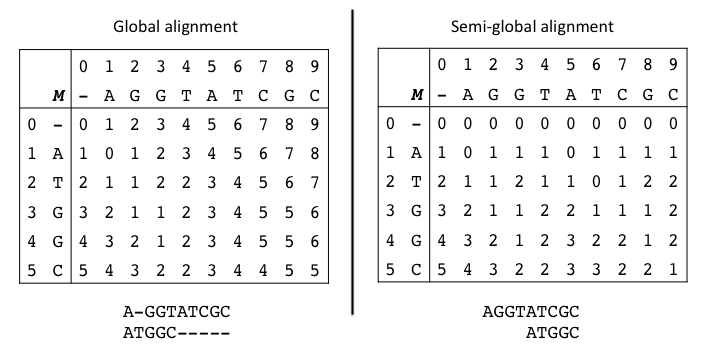
\includegraphics[width=0.7\textwidth]{global_semiglobal}
  \caption{Global vs. semi-global alignment.  In global alignments, the start and end gaps count as mismatches.  In semi-global alignments, the start and end gaps of the text are not penalized.}
  \label{fig:global_vs_semiglobal}
\end{figure}


\begin{definition}
The edit distance between a text string $t = t_1 t_2 ... t_n$ and pattern string $p = p_1 p_2  ... p_m$ is the minimum number of differences between them such that one string can be transformed into the other.
A difference is one of the following:
\begin{enumerate}

  \item A character of the text corresponds to a different character of the pattern.
  \item A character of the text corresponds to no character (a gap) in the pattern.
  \item A character of the pattern corresponds to no character (a gap) in the text.

\end{enumerate}
\end{definition}

The Needleman–Wunsch\cite{needleman_general_1970} algorithm was the first application of dynamic programming to compare sequences.
We can use this algorithm to also calculate the edit distance between two strings.
At a high level, we find the optimal alignment of two sequences by looking at the optimal alignment of the prefixes of the two sequences.

Let $M$ be an $(m+1) \times (n+1)$ table.  The value at cell $M(i,j)$ is the minimum number of edits to transform $p_1..p_i$ into $t_1..t_j$.
We can find this value by examining the three types of edits.
In the first case, lets assume we have the edit distance of aligning $p_1..p_{i-1}$ and $t_1..t_{j-1}$ (stored in $M(i-1,j-1)$) and then we add 1 edit if characters $p_i$ and $t_j$ mismatch, 0 otherwise.
The second case corresponds to aligning $p_1..p_{i-1}$ and $t_1..t_{j}$ (stored in $M(i-1,j)$) and then inserting a gap into $t$, which increases the edit distance by 1.
The final case corresponds to aligning $p_1..p_{i}$ and $t_1..t_{j-1}$ (stored in $M(i,j-1)$) and then inserting a gap into $p$, which increases the edit distance by 1.
The minimum edit distance of aligning $p_1..p_i$ and $t_1..t_j$ is the minimum of the three cases above.  These cases can be rewritten as a dynamic programming recurrence:

\begin{equation}
\begin{aligned}
M[i, j] = \quad min
\begin{cases}
\quad M[i - 1, j] + 1 \\
\quad M[i, j-1] + 1 \\
\quad M[i-1, j-1] + \begin{cases} 
0, \quad \text{if }p_i == t_j \\
1, \quad \text{else } \\
\end{cases}
\end{cases}
\end{aligned}
\end{equation}

The initial conditions of the dynamic programming table depend on whether we want the global or semi-global alignment.
Unlike with global alignment, the semi-global alignment of two strings does not penalize start and end gaps of the text (Figure \ref{fig:global_vs_semiglobal}).
For both global and semi-global alignments, $M(i,0) = i$ for $0 \leq i \leq m$.
Global alignment penalizes start gaps in the text, so $M(0,i) = i$ for $0 \leq i \leq n$.
For semi-global alignment, $M(0,i) = 0$ for $0 \leq i \leq n$.

Once the dynamic programming table $M$ is populated, we need to specify where to find the solution, i.e., the minimum edit distance between the pattern and text.
In the case of global alignment, the solution will be located in cell $M(m,n)$.
For semi-global alignments, we do not penalize end gaps in the text, so the solution lies in the cell that contains the minimum value of row $m$ of $M$. Thus, the final algorithm:

% Edit distance computation
 \begin{algorithm}
 \caption{Compute global edit distance between two strings. $O(nm)$ work.}\label{edit_distance}
 \begin{algorithmic}[1]
 \Procedure{ComputeEditDistance}{$text,pattern$}
 \State $n\gets |text|$
 \State $m\gets |pattern|$

 \For{$i=0 .. m$}   \State $M(i,0) \gets i$ \EndFor
 \For{$i=0 .. n$}
  \State $M(0,i) \gets i$
\EndFor

 \For{$i=1 .. n$}
 \For{$j=1 .. m$}
  \State $row \gets M(i-1,j) + 1$ \Comment Number of edits with a gap inserted into $b$
  \State $col \gets M(i,j-1) + 1$ \Comment Number of edits with gap inserted into $a$
  \State $diag \gets M(i-1, j-1)$ \Comment Number of edits with matching characters $a_i$ and $b_j$
  \If{$a_i \neq b_j$}  $diag \gets diag +  1$ \EndIf
  \State $M(i,j) \gets \text{min}(row,col,diag)$
\EndFor
\EndFor
\Return $M(n,m)$
\EndProcedure
\end{algorithmic}
\end{algorithm}

Since we are populating a table with $(m+1) \times (n+1)$ values and doing a constant amount of work per cell (looking up the value of three adjacent cells) the total time and space requirement to calculate the edit distance between two strings is $O(nm)$.
The space requirement can be relaxed to $O(n)$ using a divide-and-conquer approach\cite{gusfield_algorithms_1997}.
Similarly, if we set a bounds on the maximum number of edits ($k$), we can reduce the runtime even further.
If we want to find a global alignment within $k$-differences (edits), we only need to worry about a $2k+1$ band along the diagonal.
This reduces the time complexity from $O(nm)$ to $O(nk)$.
However, this assumes we are aligning the two sequences end-to-end.
In the section, we will outline the steps necessary to reduce this to $O(nk)$ for semi-global alignments.

%Algorithms for $k-mismatches$ only satisfies differences of type 1.

%Algorithm to solve $k$-differences 

